% !TEX root = ../main.tex
% --+ 10.41 RG-F Experiment +---------------------------------------------------
\begin{frame}{Run Group F (RG-F) Experiment}
    \label{10.41::rgf_experiment}

    \begin{itemize}
        \item
            The RG-F experiment ran at Hall B during \ef{Spring} and \ef{Summer 2020}.

        \vspace{12pt}
        \item
            Its target is composed of a D2 gas at room temperature.

        \vspace{12pt}
        \item
            The RG-F target is 55 cm long in $z$, \ef{allowing us to compare acceptance across the scattering chamber}.
    \end{itemize}

    \vspace{-6pt}

    \begin{center}
        \begin{figure}[t]
            \centering{
                \fbox{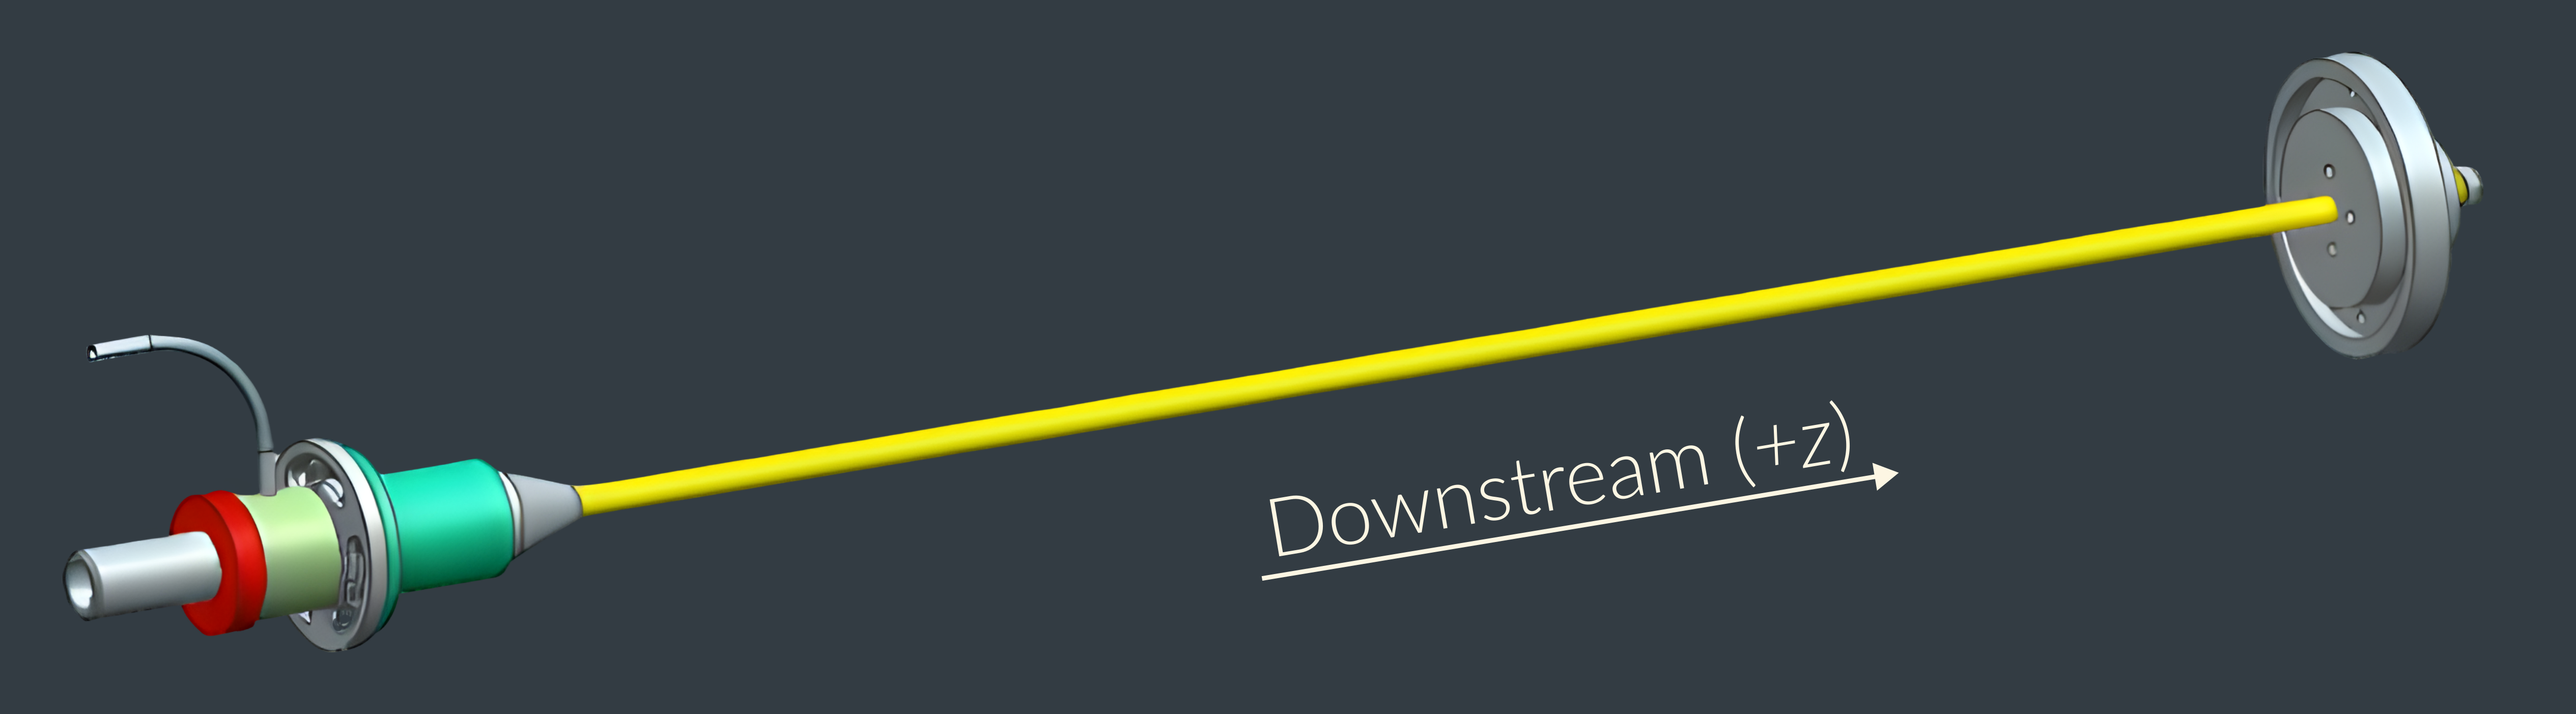
\includegraphics[width=0.8\textwidth]{41bonus_target.png}}
            }
        \end{figure}
    \end{center}

    \vspace{-6pt}

    \scriptsize{\textit{
        \ef{RG-F target CAD render.}
        Leftmost is a glass window of the scattering chamber, and the gas target is held at both sides by aluminium walls.
    }}
\end{frame}
